\subsection{Vista para el adminstrador}\label{subsec5.1.2}

\subsubsection{Productos y pedidos}\label{subsec5.1.2.1}
En la vista de gestión de productos, en la parte superior derecha se encuentra un botón que permite añadir un nuevo producto al catálogo. Debajo de este, se muestran todos los productos disponibles, cada uno con su información relevante, como nombre, precio y categoría. Junto a cada producto, el administrador dispone de botones para eliminar el producto, editarlo, y dos botones adicionales para marcar o desmarcar el producto como novedad o como liquidación, facilitando la organización y promoción del inventario.

\begin{figure}[H]
\begin{center}
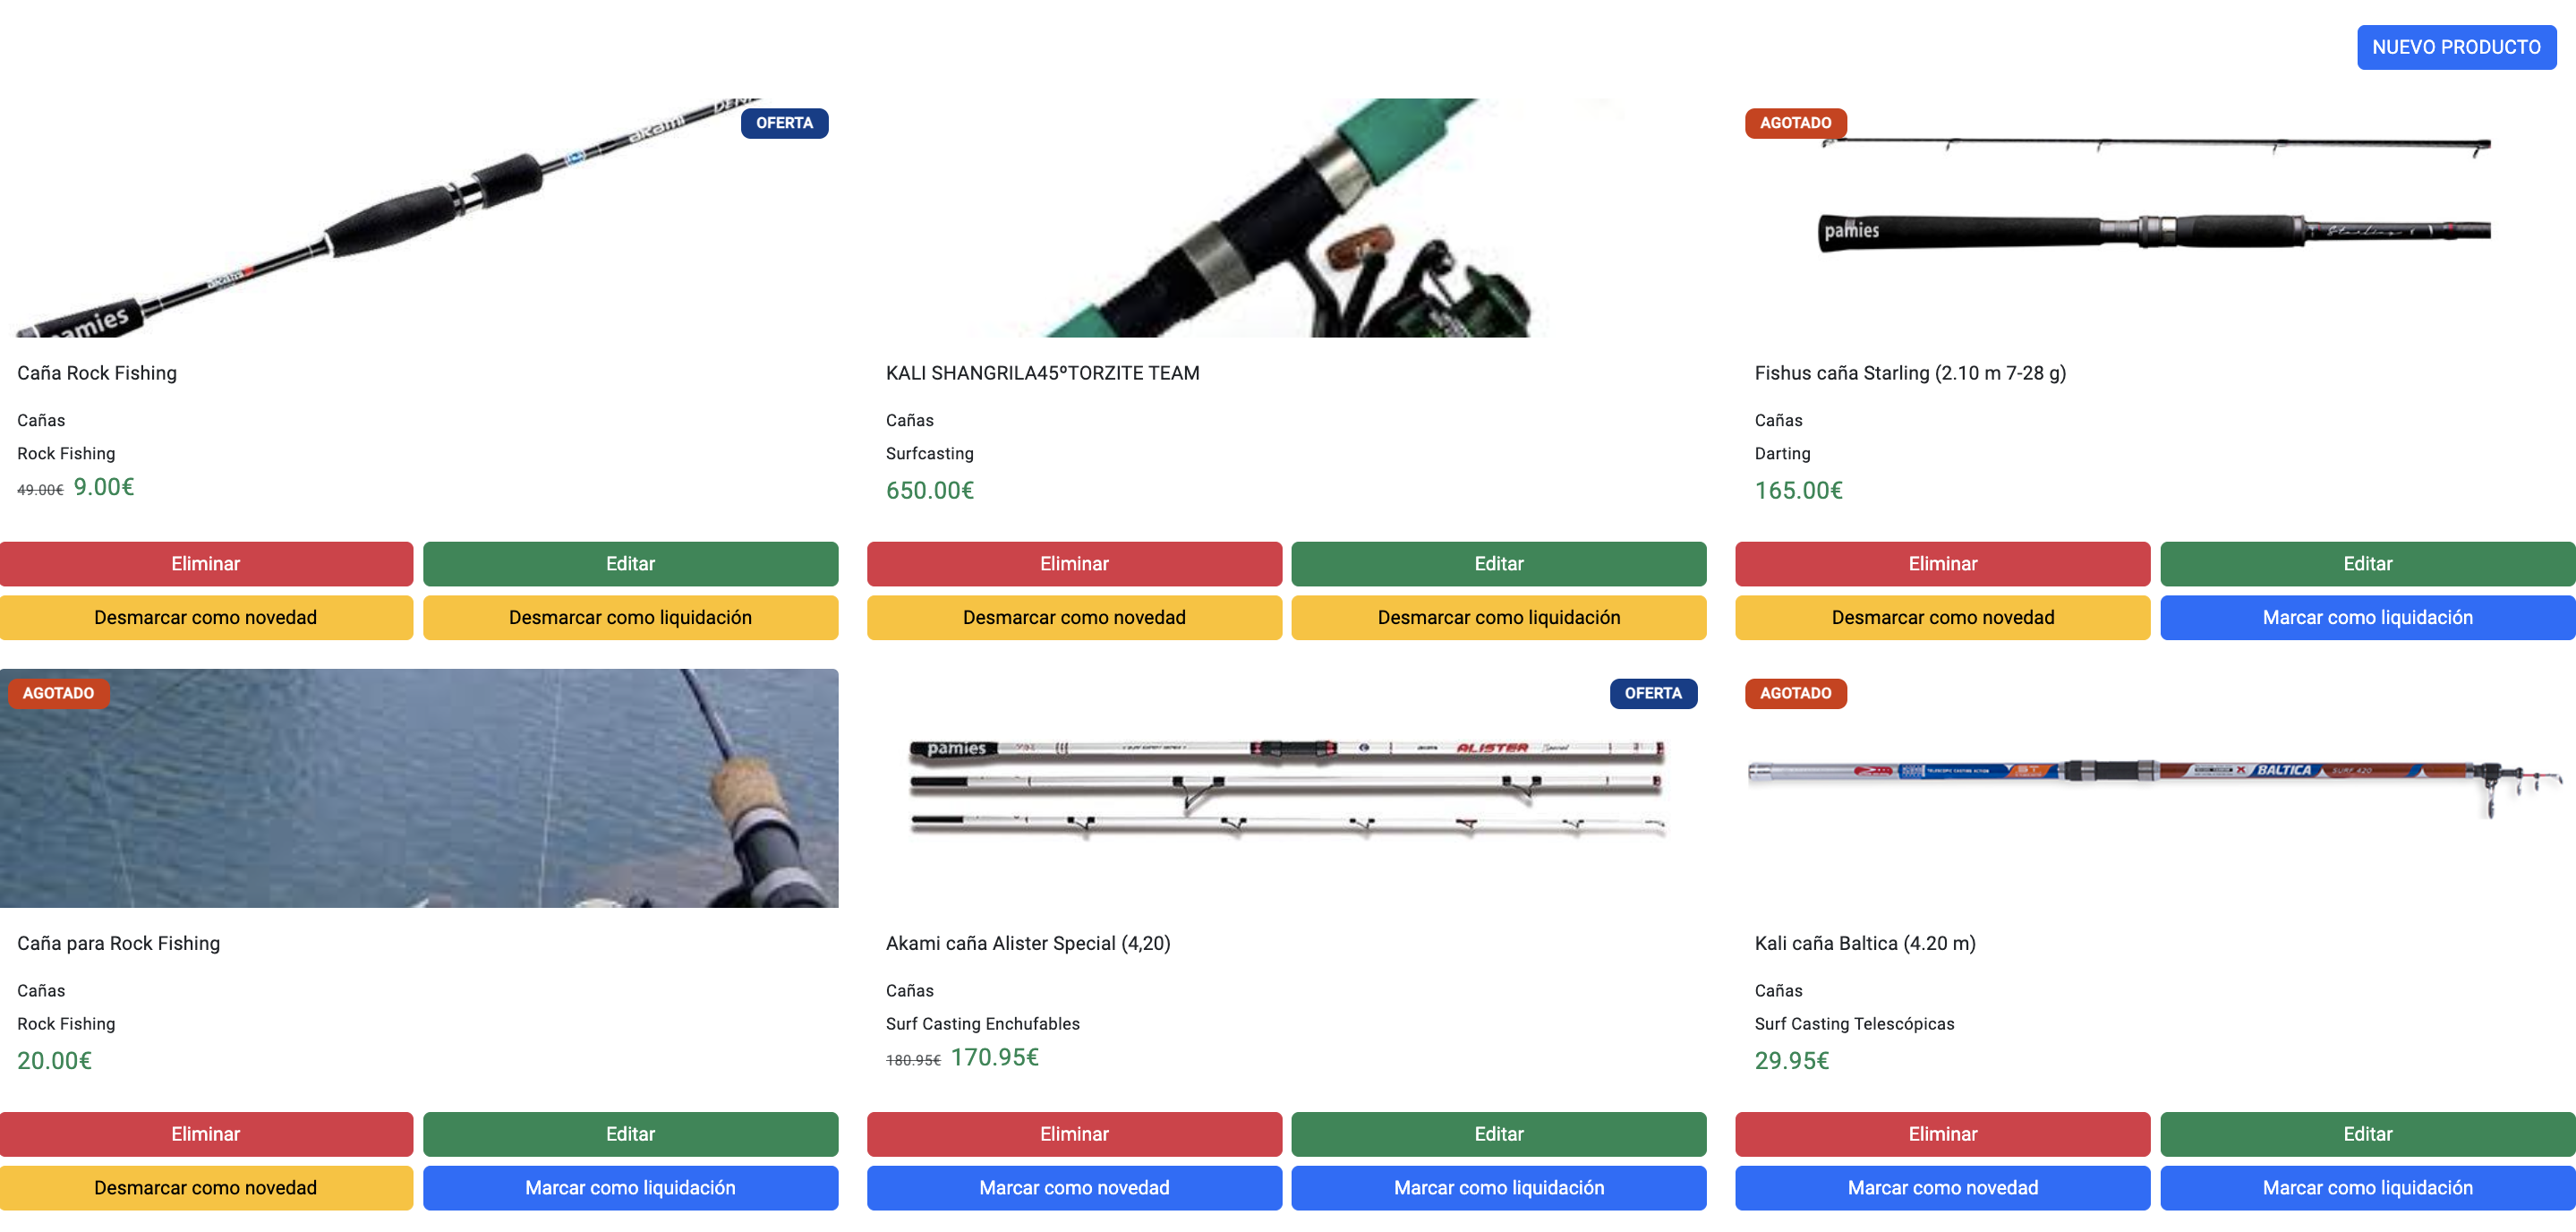
\includegraphics[scale=0.35]{./Images/vistaAdminProductos.png}
\caption{Vista Gestión de productos} Fuente: Elaboración propia.

\label{fig:fig1}

\end{center}
\end{figure}

Cuando se desea añadir un nuevo producto, se muestra un formulario en el que se deben completar todos los campos necesarios para crear el producto, como su nombre, precio, descripción, categoría, etc. Además, se incluye un campo para subir la imagen principal del producto, así como un campo adicional para añadir imágenes secundarias que ayuden a mostrar el producto desde diferentes ángulos o contextos.

\begin{figure}[H]
\begin{center}
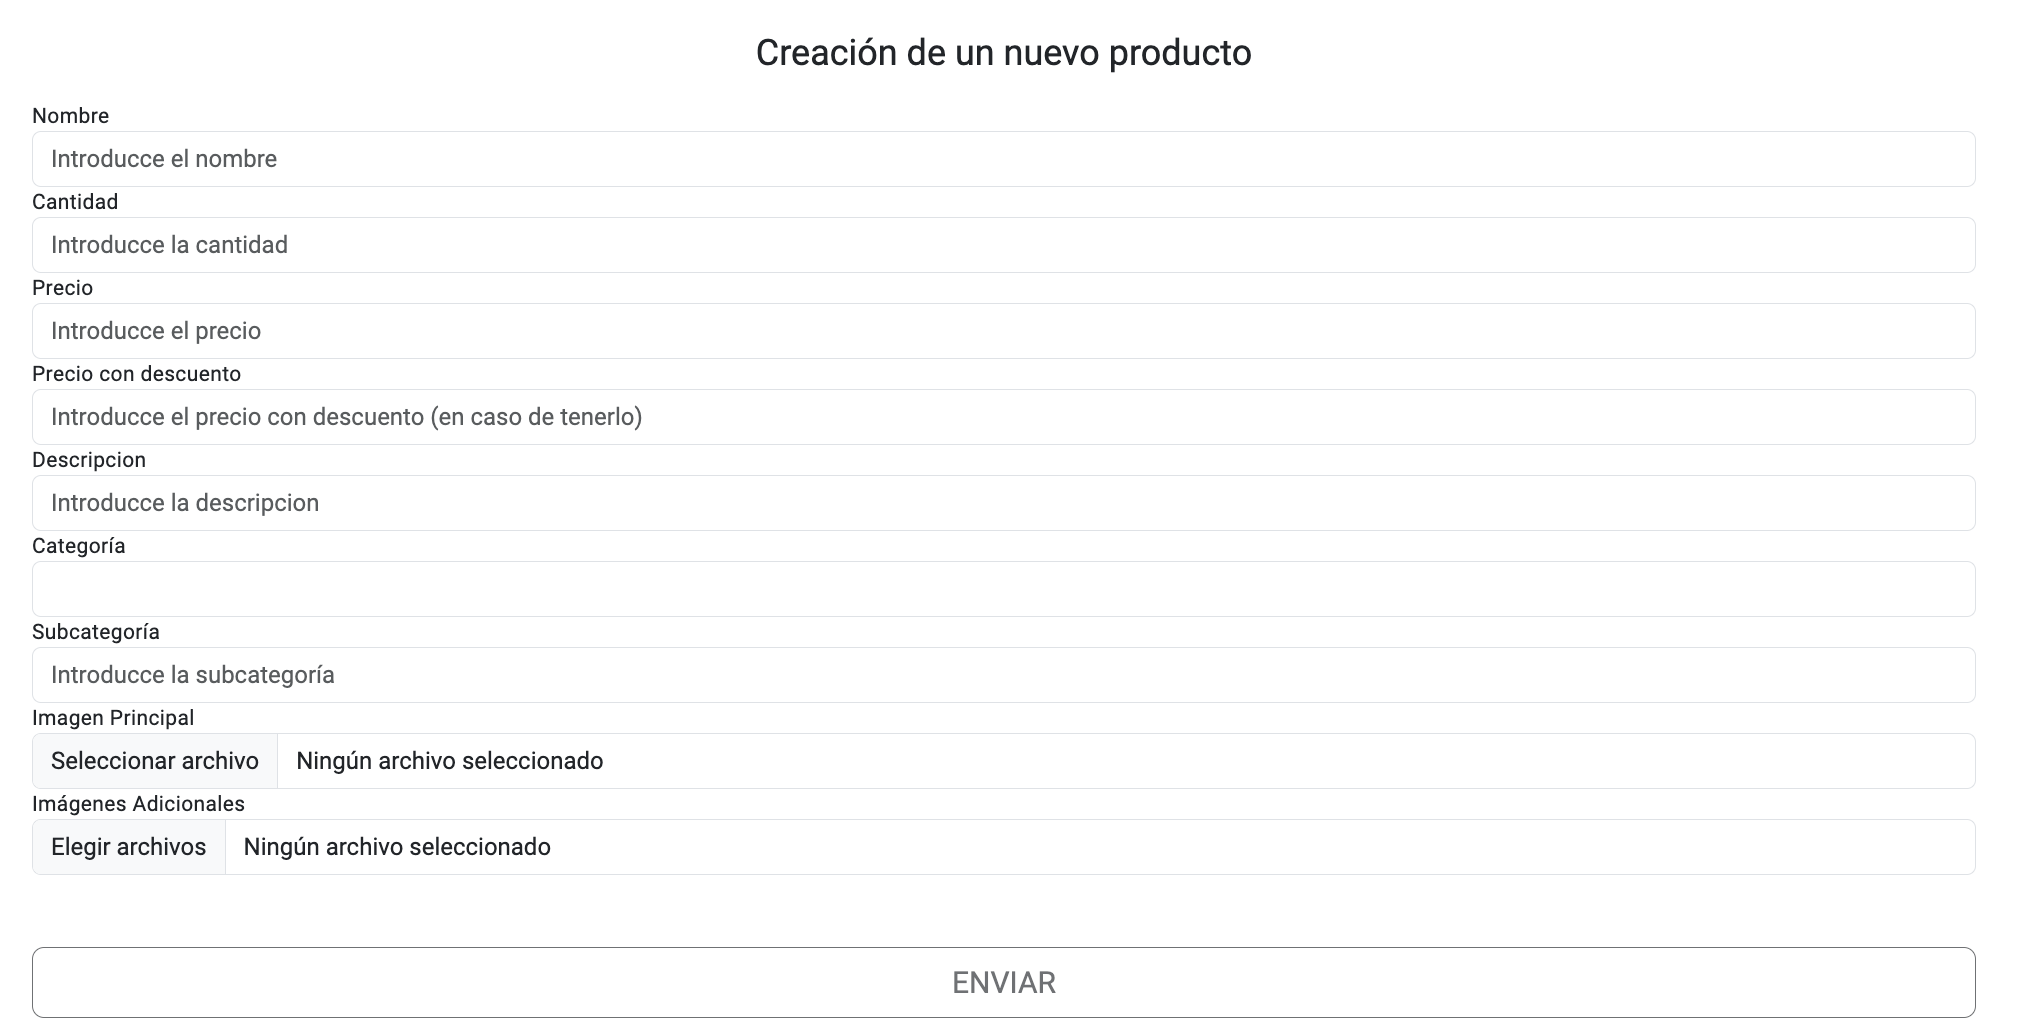
\includegraphics[scale=0.5]{./Images/vistaAdminNuevoProducto.png}
\caption{Vista Nuevo producto} Fuente: Elaboración propia.

\label{fig:fig1}

\end{center}
\end{figure}

En el caso de editar un producto existente, el administrador accede al mismo formulario de creación, pero esta vez aparece rellenado con los datos actuales del producto que se desea modificar. Aquí se pueden ajustar todos los detalles del producto, incluyendo su imagen principal y las imágenes adicionales, para mantener el catálogo actualizado.

\vspace{0.5cm}

Por último, en el apartado de gestión de pedidos, se muestra una lista con todos los pedidos realizados, incluyendo el número de pedido, el nombre del cliente, su teléfono y correo electrónico, la cantidad de productos, los productos solicitados, y el precio total del pedido. Además, se puede utilizar un buscador para filtrar los pedidos por cliente, permitiendo ver rápidamente todos los pedidos que ha realizado un cliente en particular.

\begin{figure}[H]
\begin{center}
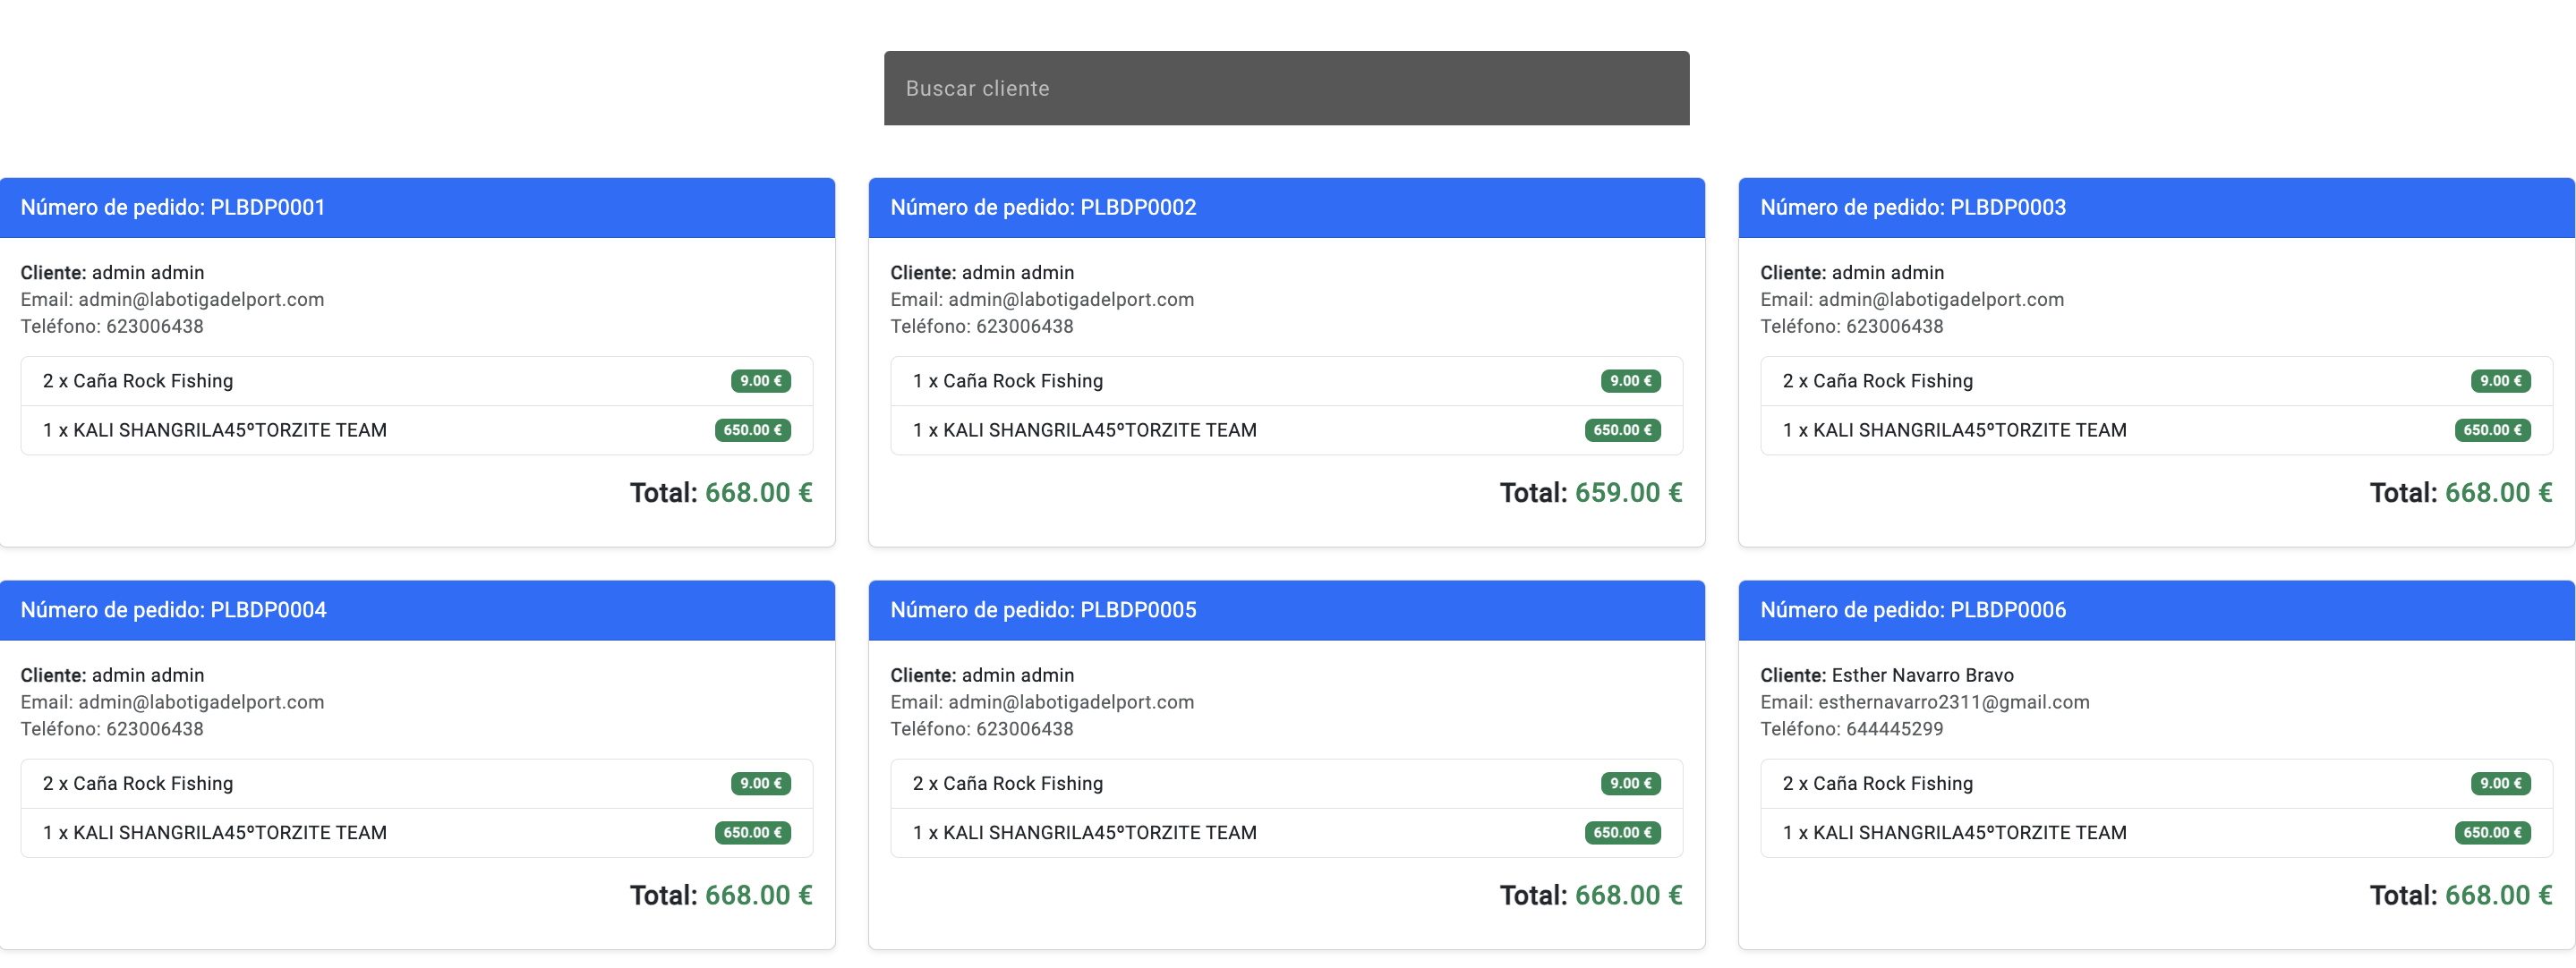
\includegraphics[scale=0.35]{./Images/vistaAdminPedidos.png}
\caption{Vista Nuevo producto} Fuente: Elaboración propia.

\label{fig:fig1}

\end{center}
\end{figure}

\subsubsection{Reserva de cebo}\label{subsec5.1.2.2}
La vista de gestión de reservas de cebo para el administrador presenta una pantalla donde se listan todas las reservas de cebo realizadas por los clientes. En la parte superior, se incluye un buscador que permite filtrar las reservas por el nombre del cliente, mostrando solo las relacionadas con dicho usuario. Además, se han implementado pestañas (tabs) que permiten al administrador alternar entre las reservas "todas", "futuras" o "pasadas", facilitando la organización y visualización de las mismas.

\vspace{0.5cm}

En cada reserva se muestra información clave, como el número de reserva, la fecha de recogida, los datos básicos del cliente (como nombre, teléfono y correo electrónico), así como una lista detallada de los productos reservados con sus respectivas cantidades y precios. Junto a cada reserva, se incluyen dos botones de acción: uno para eliminar la reserva si es necesario, y otro para marcar la reserva como recogida, actualizando así el estado de la misma en el sistema.

\begin{figure}[H]
\begin{center}
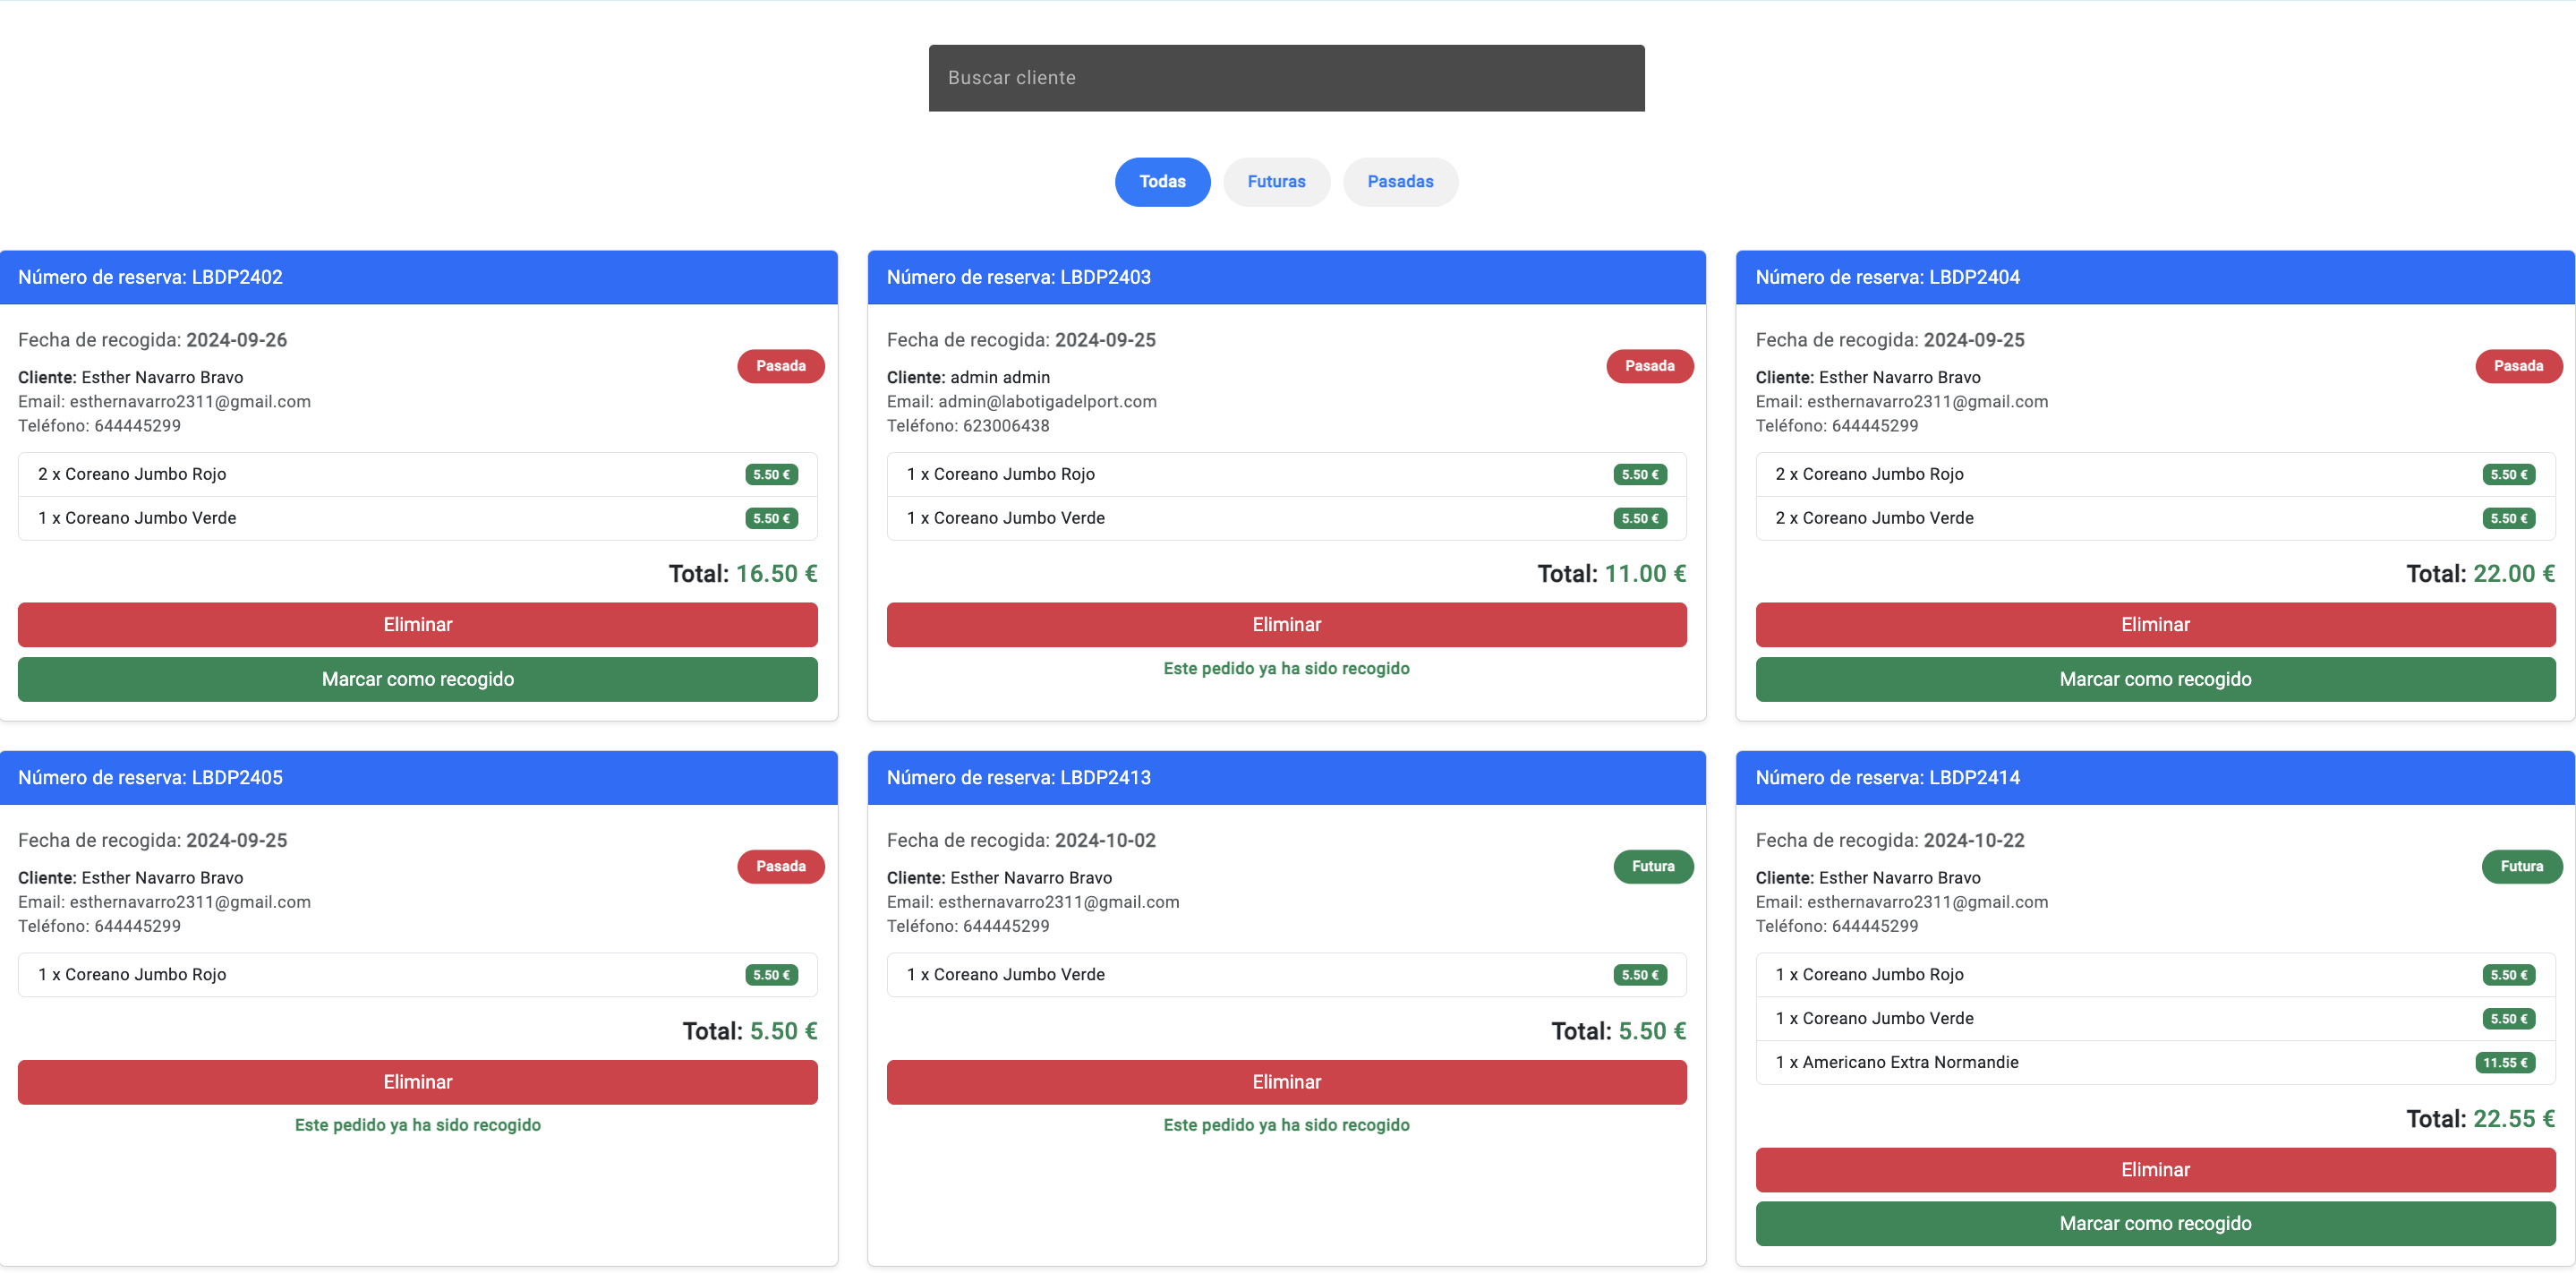
\includegraphics[scale=0.30]{./Images/vistaAdminReservas.png}
\caption{Vista gestión de reserva de cebo} Fuente: Elaboración propia.

\label{fig:fig1}

\end{center}
\end{figure}


\subsubsection{Página principal}\label{subsec5.1.2.3}

En la página principal del administrador, se ofrece la posibilidad de modificar y gestionar los tres módulos clave visibles para los clientes. El primer módulo es el banner informativo, donde el administrador puede crear un nuevo banner, editarlo, eliminarlo o marcarlo como principal para que sea el que aparezca de manera destacada en la página principal. Esto permite un control flexible sobre las promociones o enlaces que se quieran resaltar en la tienda.

\begin{figure}[H]
\begin{center}
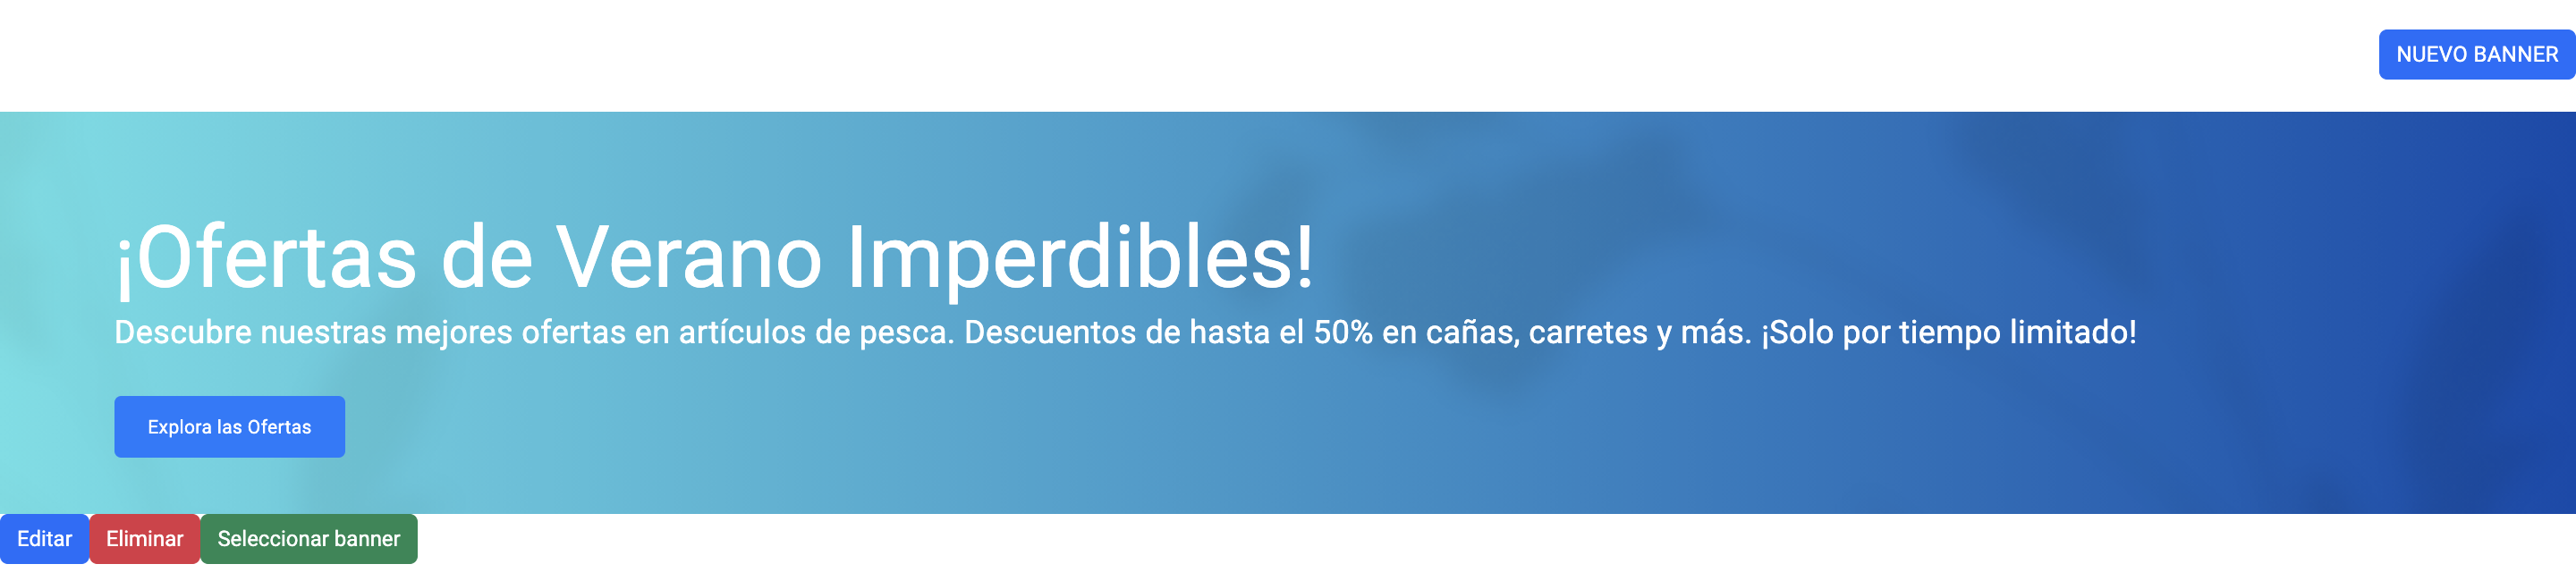
\includegraphics[scale=0.35]{./Images/vistaAdminBanner.png}
\caption{Gestión del banner informativo} Fuente: Elaboración propia.

\label{fig:fig1}

\end{center}
\end{figure}

El segundo módulo corresponde al carrusel de productos más vendidos, pero en realidad, el administrador tiene la libertad de seleccionar manualmente los productos que desea que aparezcan en este carrusel. El límite es de seis productos, y si se intenta seleccionar más, el sistema no lo permite y se muestra un mensaje de advertencia para alertar al administrador de que ha alcanzado el máximo permitido.

\begin{figure}[H]
\begin{center}
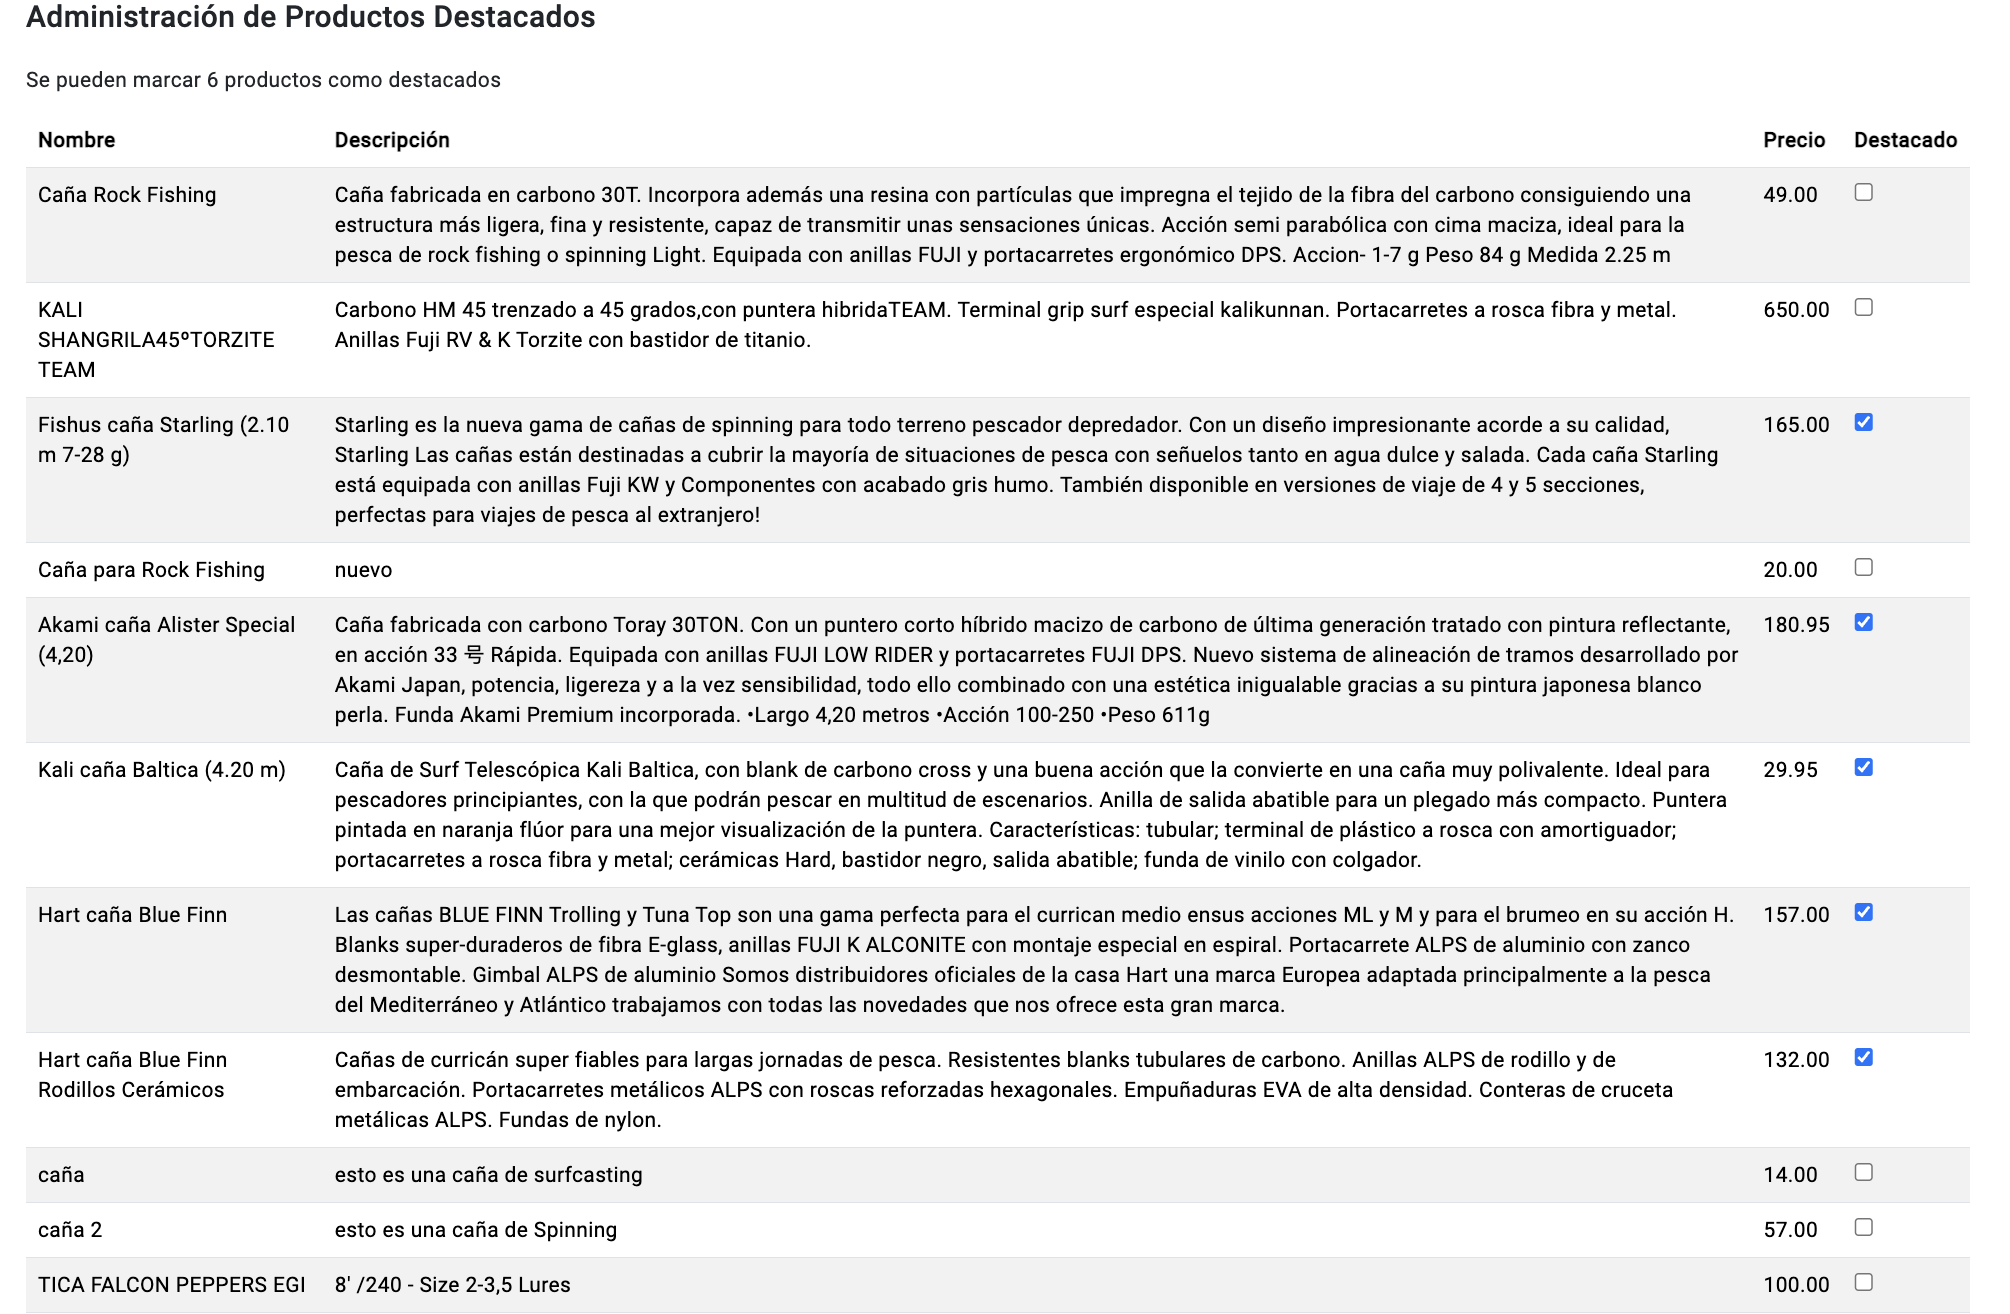
\includegraphics[scale=0.50]{./Images/vistaAdminCarrusel.png}
\caption{Gestión del carrusel de productos} Fuente: Elaboración propia.

\label{fig:fig1}

\end{center}
\end{figure}

El tercer módulo corresponde a las cards de novedades, ofertas y liquidaciones. Cada una de estas tarjetas redirige a una página específica. La tarjeta de novedades lleva a la página de productos marcados como novedades, los cuales se gestionan desde la sección de productos, donde los productos pueden ser marcados o desmarcados como novedades según la decisión del administrador. De manera similar, la tarjeta de liquidaciones lleva a la página de productos en liquidación, y estos también pueden ser marcados o desmarcados como productos en liquidación desde la gestión de productos.

\vspace{0.5cm}

En el caso de la tarjeta de ofertas, esta redirige a la página de productos que tienen precios con descuento. Los productos que se muestran aquí son aquellos que el administrador ha configurado con algún tipo de descuento en su precio.

\begin{figure}[H]
\begin{center}
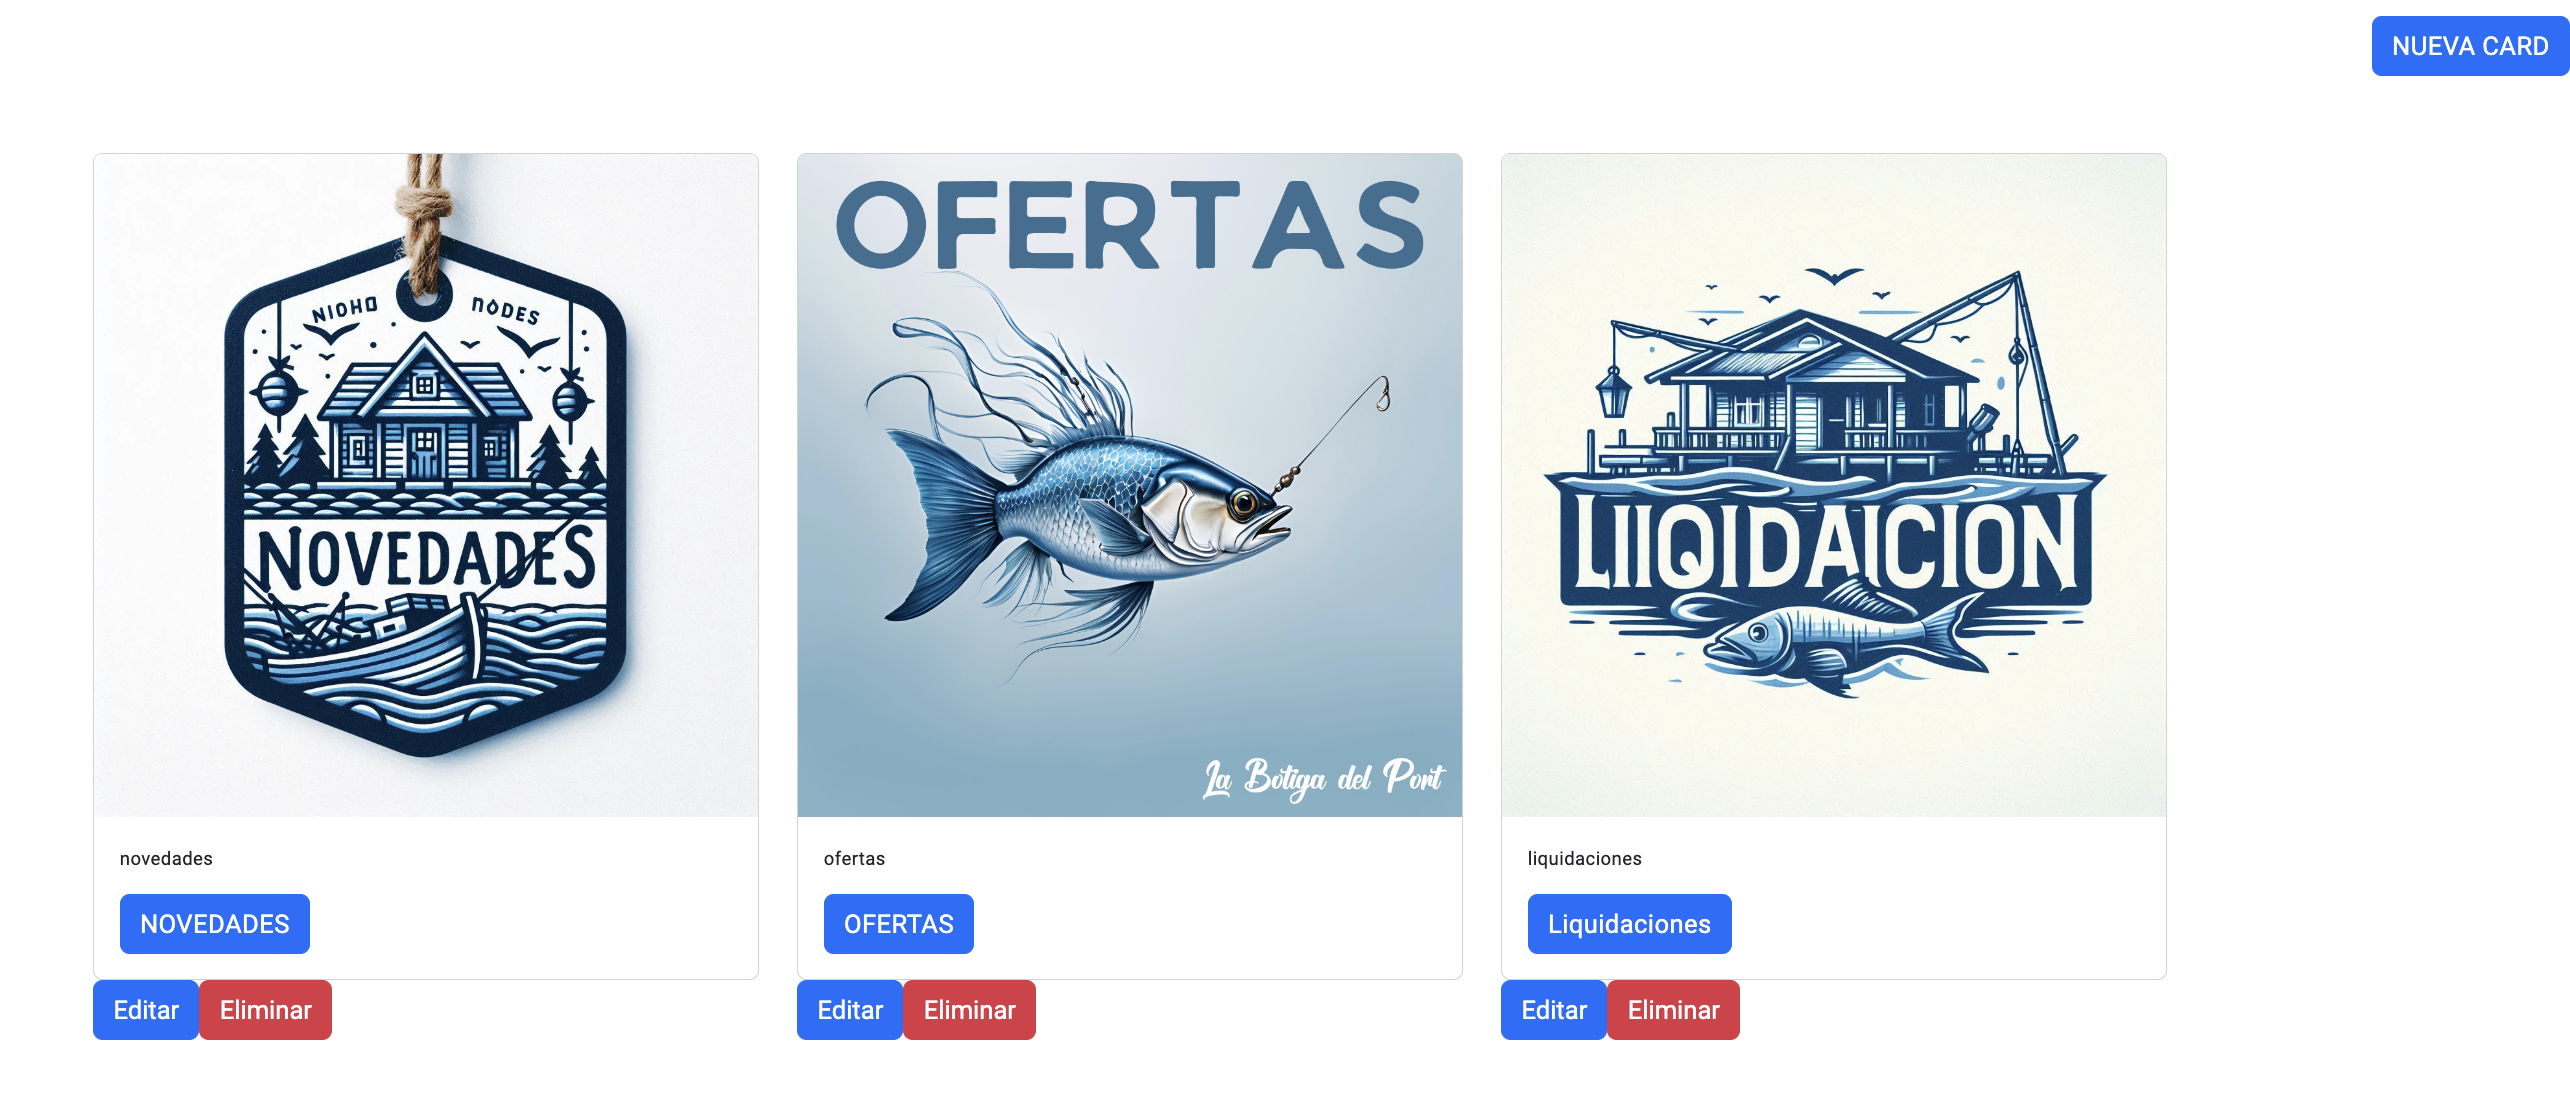
\includegraphics[scale=0.35]{./Images/vistaAdminCards.png}
\caption{Gestión de tarjetas} Fuente: Elaboración propia.

\label{fig:fig1}

\end{center}
\end{figure}

\subsubsection{Códigos de descuento}\label{subsec5.1.2.4}
En esta vista, el administrador puede visualizar todos los códigos de descuento creados hasta el momento. Para cada código, se muestra información clave como el nombre del código, el porcentaje de descuento aplicado, la fecha de inicio y la fecha de finalización del descuento. Además, junto a cada código se incluye una etiqueta que indica si el código está "activo" o si ha pasado su fecha de validez. Junto a estos datos, el administrador dispone de opciones para editar o eliminar cualquier código de descuento existente.

\vspace{0.5cm}

En la parte superior de la vista, se encuentra un botón para crear un nuevo código de descuento. Al seleccionarlo, el administrador deberá completar un formulario que solicita la misma información que se muestra en la lista, es decir, nombre del código, porcentaje de descuentoy fechas de inicio y fin.

\begin{figure}[H]
\begin{center}
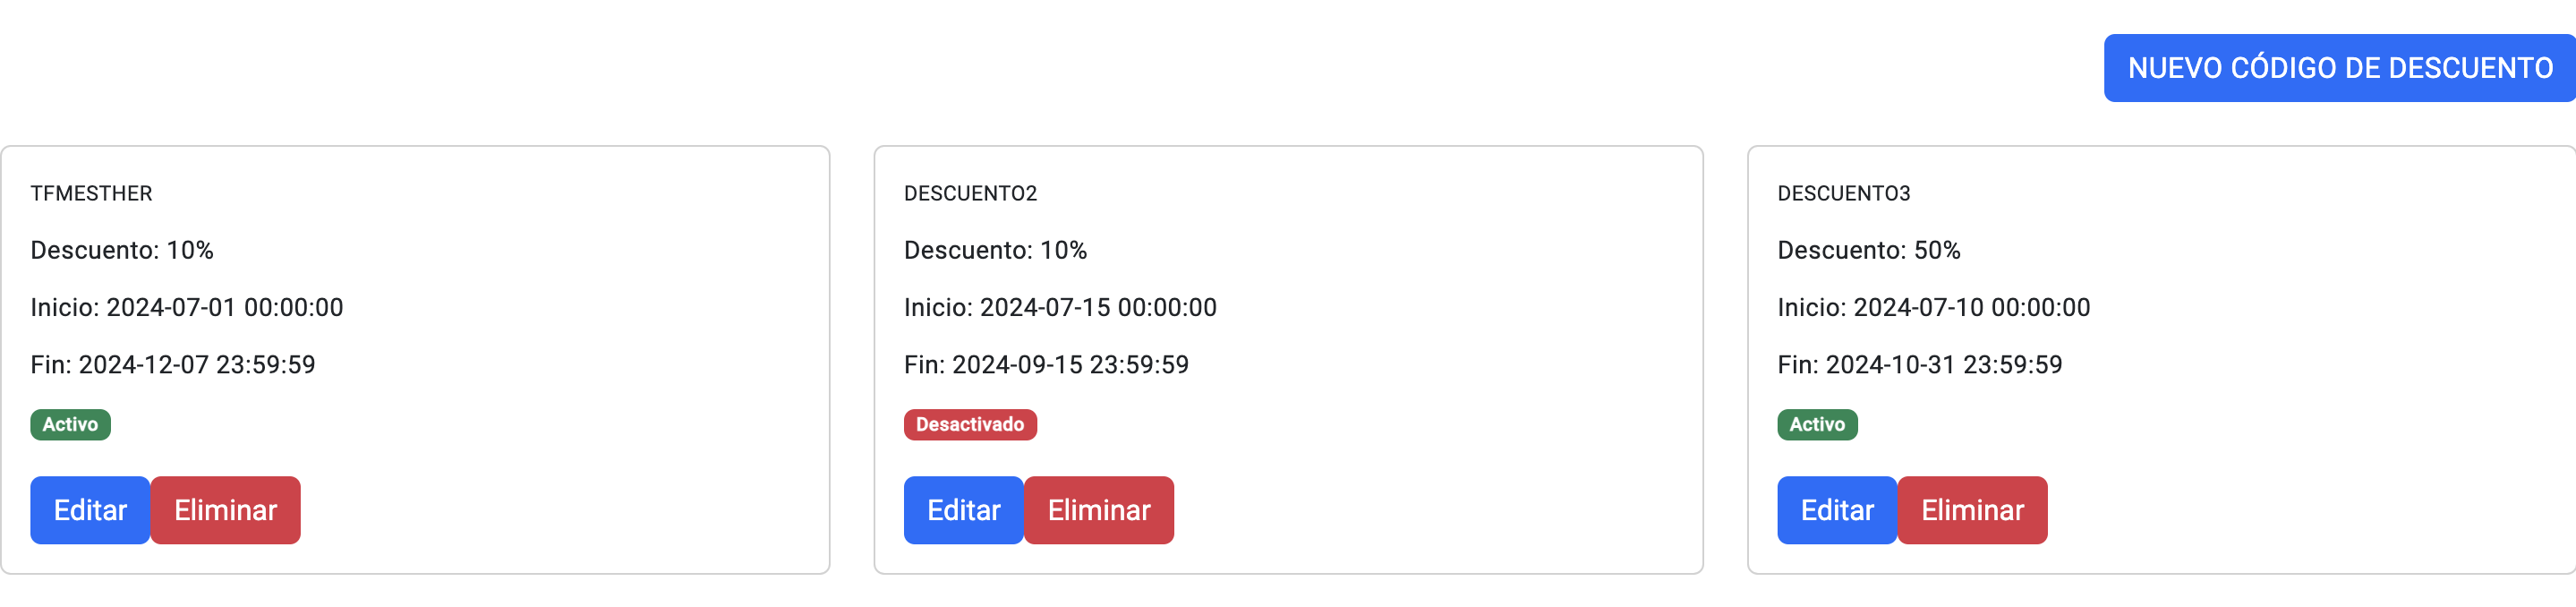
\includegraphics[scale=0.3]{./Images/vistaAdminCodigo.png}
\caption{Vista Códigos de descuento} Fuente: Elaboración propia.

\label{fig:fig2}

\end{center}
\end{figure}

\subsection{Ubicación}\label{subsec5.1.3}

En esta sección, se presenta la vista de la ubicación de La Botiga del Port a través de un mapa interactivo. Esta visualización ha sido posible gracias a la integración de OpenStreetMap, una plataforma de mapeo colaborativa y de código abierto que permite acceder a mapas detallados y actualizados. Los usuarios pueden explorar la ubicación exacta del establecimiento, facilitando su visita y mejorando la experiencia del cliente.

\begin{figure}[H]
\begin{center}
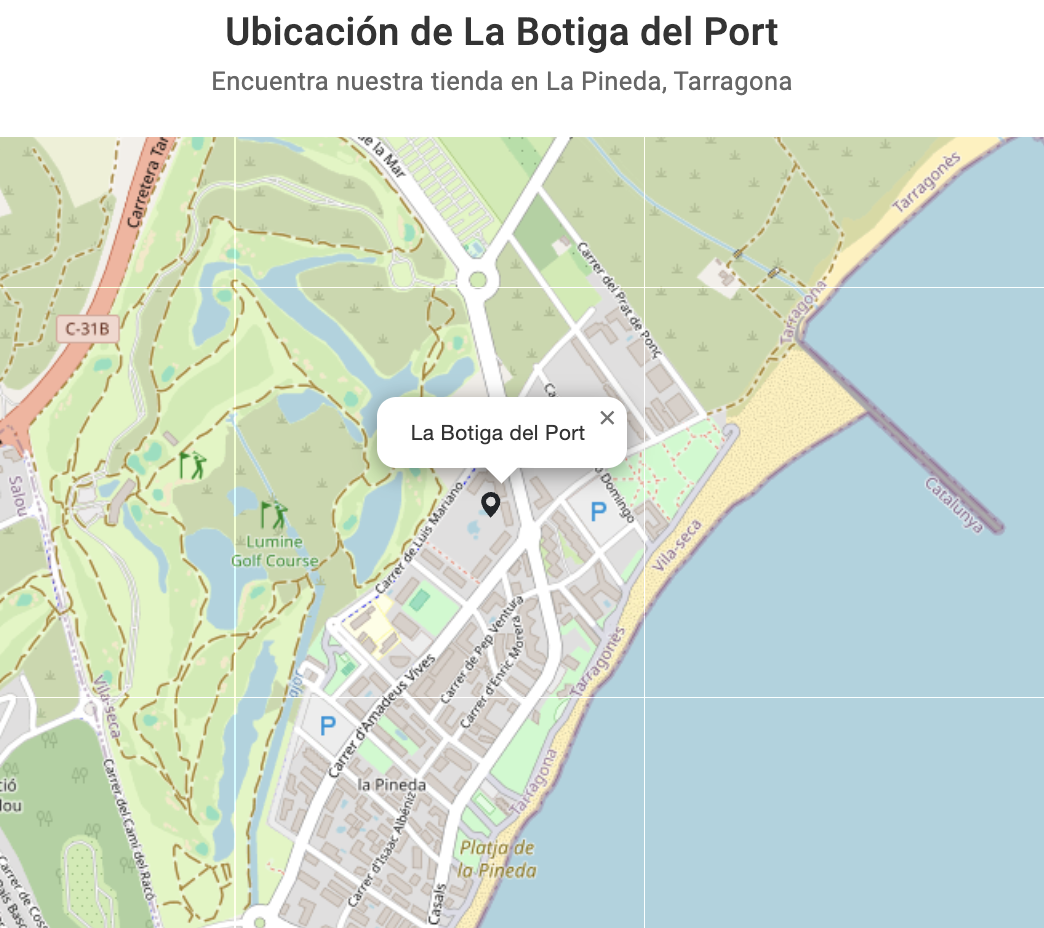
\includegraphics[scale=0.5]{./Images/ubicacion.png}
\caption{Vista de la ubicación} Fuente: Elaboración propia.

\label{fig:fig2}

\end{center}
\end{figure}

\subsection{Navegación en desktop y mobile}\label{subsec5.1.4}
Las vistas de navegación en desktop y mobile están diseñadas de manera diferente para adaptarse a cada tipo de dispositivo, garantizando una experiencia de usuario fluida y optimizada. Mientras que en la versión de escritorio la información se presenta de forma más amplia y accesible en todo momento, en la versión móvil se prioriza la simplicidad y la accesibilidad a través de menús desplegables.

\vspace{0.5cm}

En la versión de escritorio, la navegación se estructura en un header que contiene varios elementos clave. A la izquierda se encuentra el logo de la página, seguido de un buscador central para facilitar la búsqueda rápida de productos. A la derecha se incluyen los botones de login para acceder a la cuenta y el carrito, donde los usuarios pueden visualizar los productos seleccionados. Justo debajo del header, se muestra una barra de navegación con las diferentes categorías de productos. Al hacer clic en una categoría, se despliegan las subcategorías correspondientes, permitiendo una navegación rápida y organizada a través del catálogo.

\begin{figure}[H]
\begin{center}
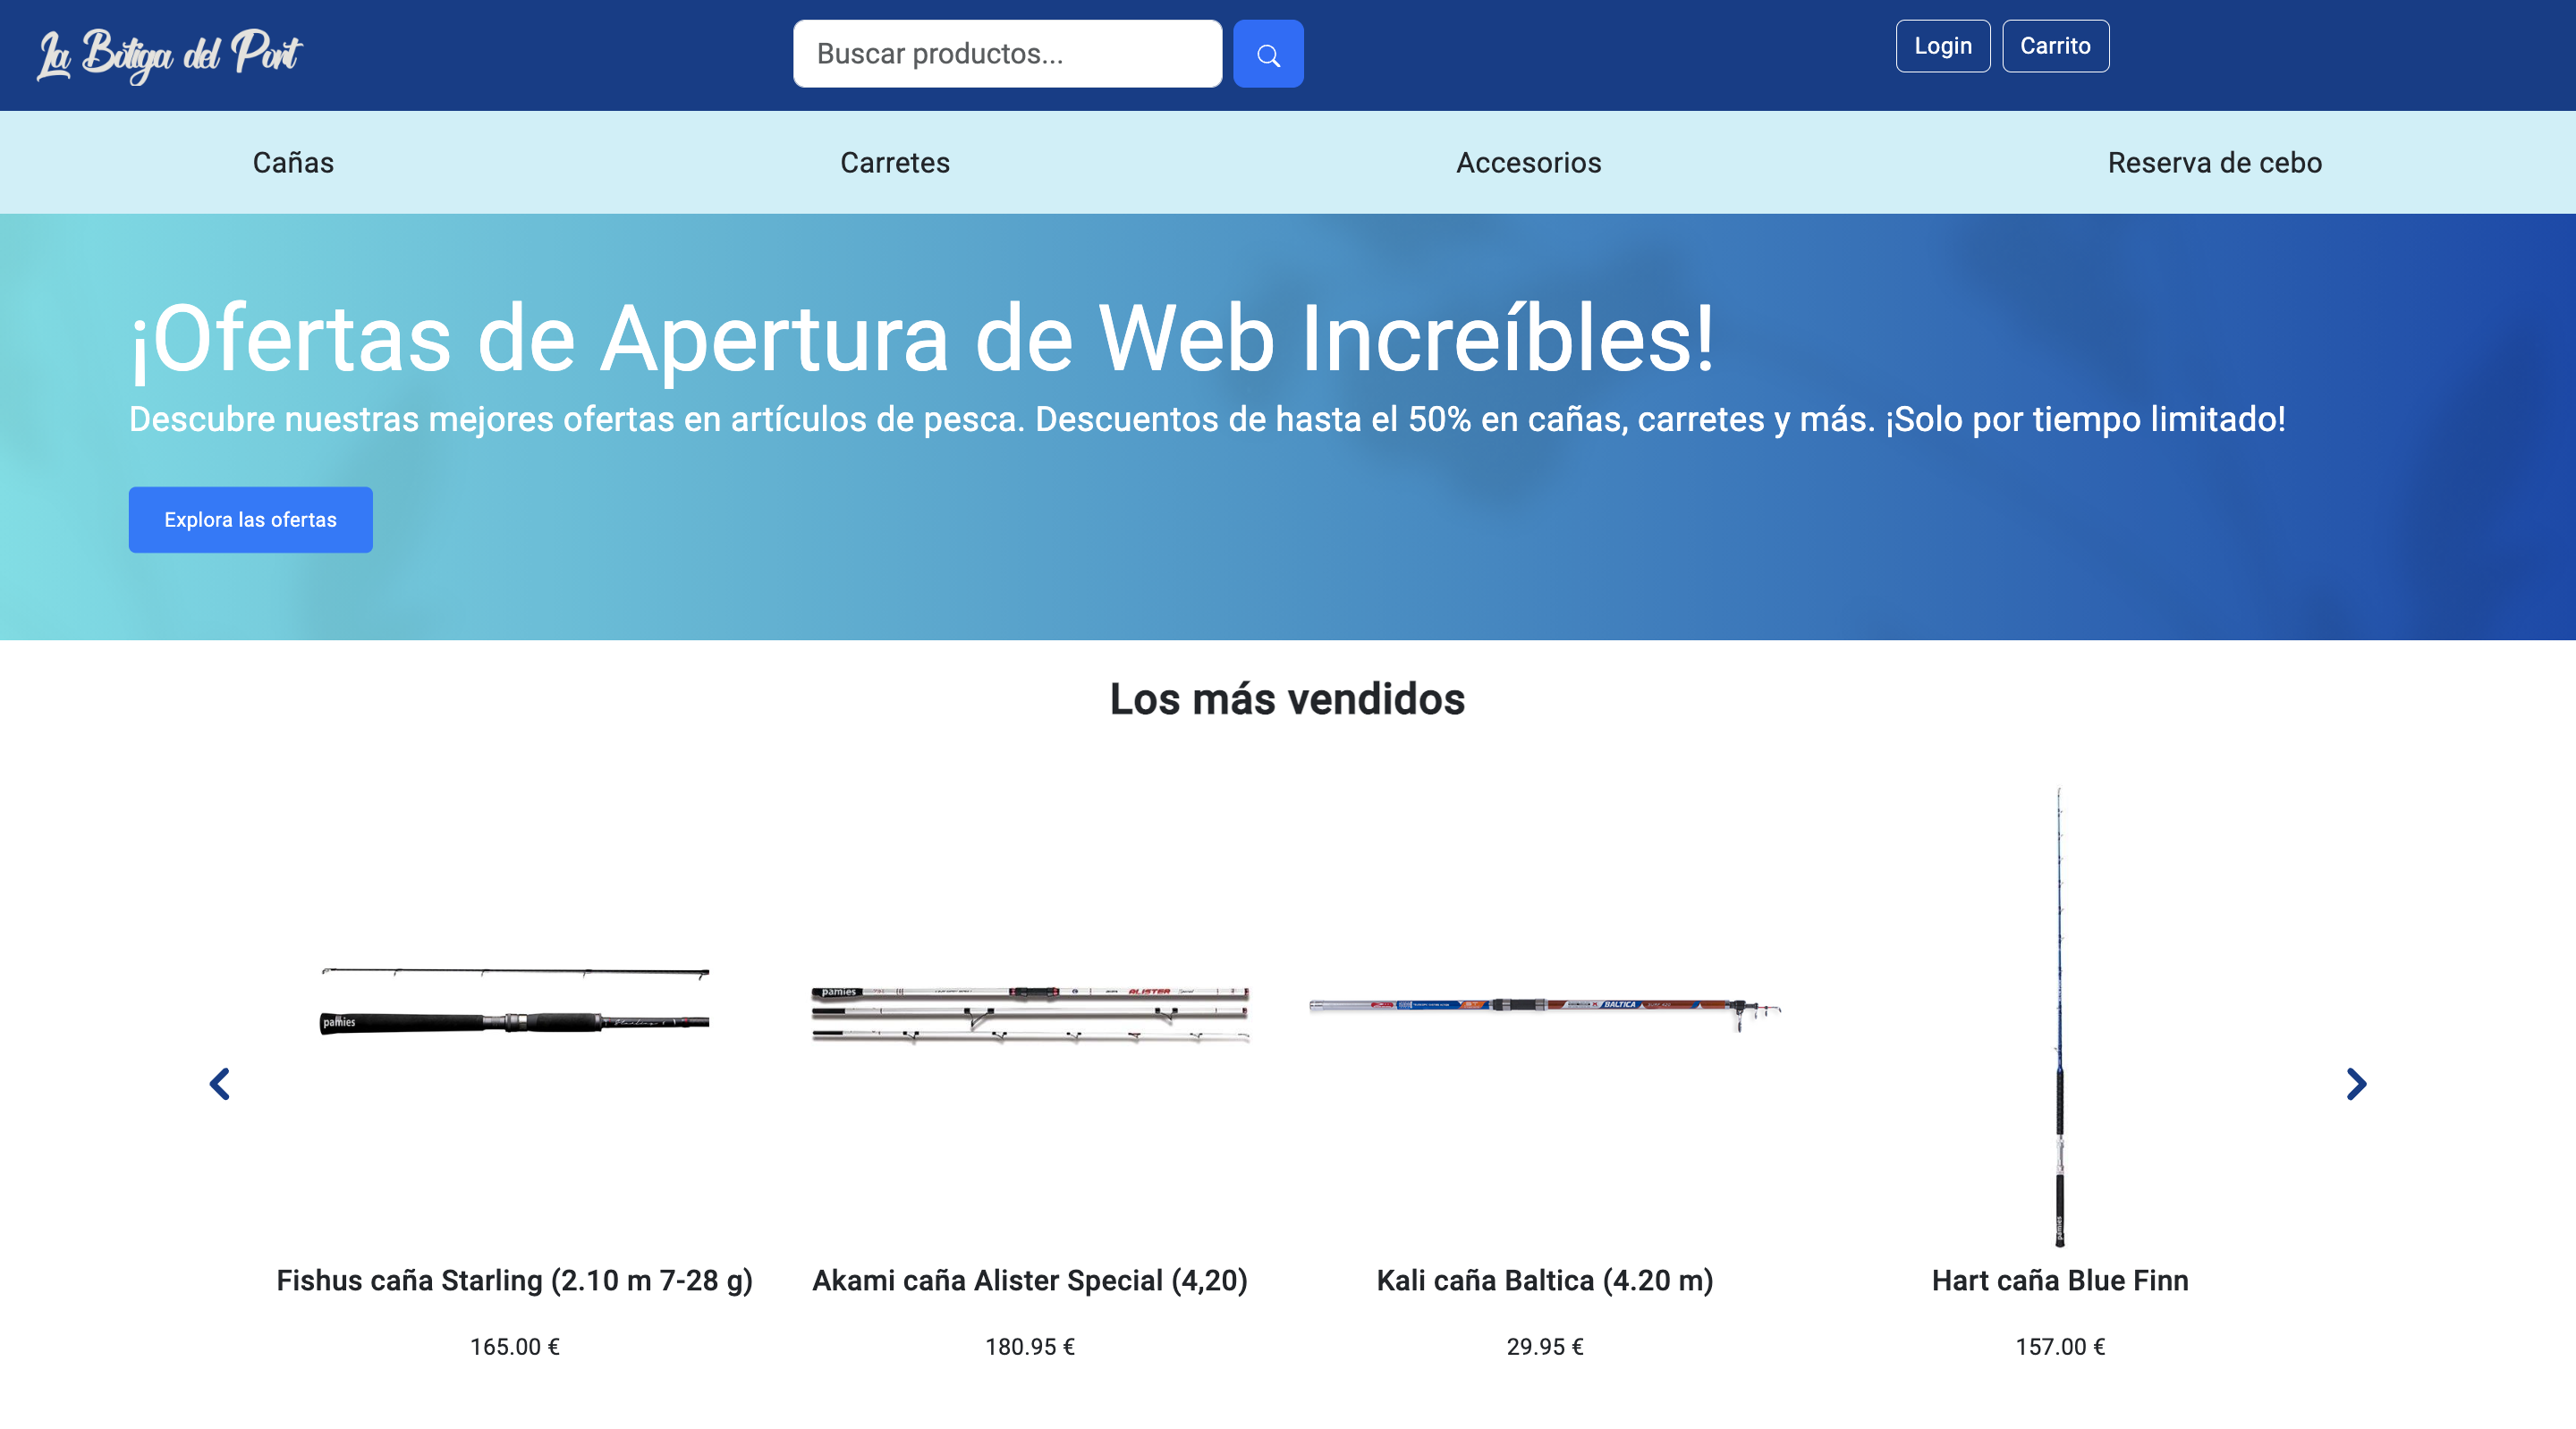
\includegraphics[scale=0.3]{./Images/vistaDesktop.png}
\caption{Vista general en desktop} Fuente: Elaboración propia.

\label{fig:fig2}

\end{center}
\end{figure}

En dispositivos móviles, la navegación está optimizada para pantallas más pequeñas. En la parte superior, solo se muestran el logo y un icono de menú hamburguesa que, al abrirse, despliega un menú lateral. En este menú, el usuario puede acceder al buscador, a los botones de login y carrito, y visualizar todas las categorías de productos. Al seleccionar una categoría, se despliegan las subcategorías relacionadas, permitiendo una navegación clara y eficiente en dispositivos móviles.

\begin{figure}[H]
\begin{center}
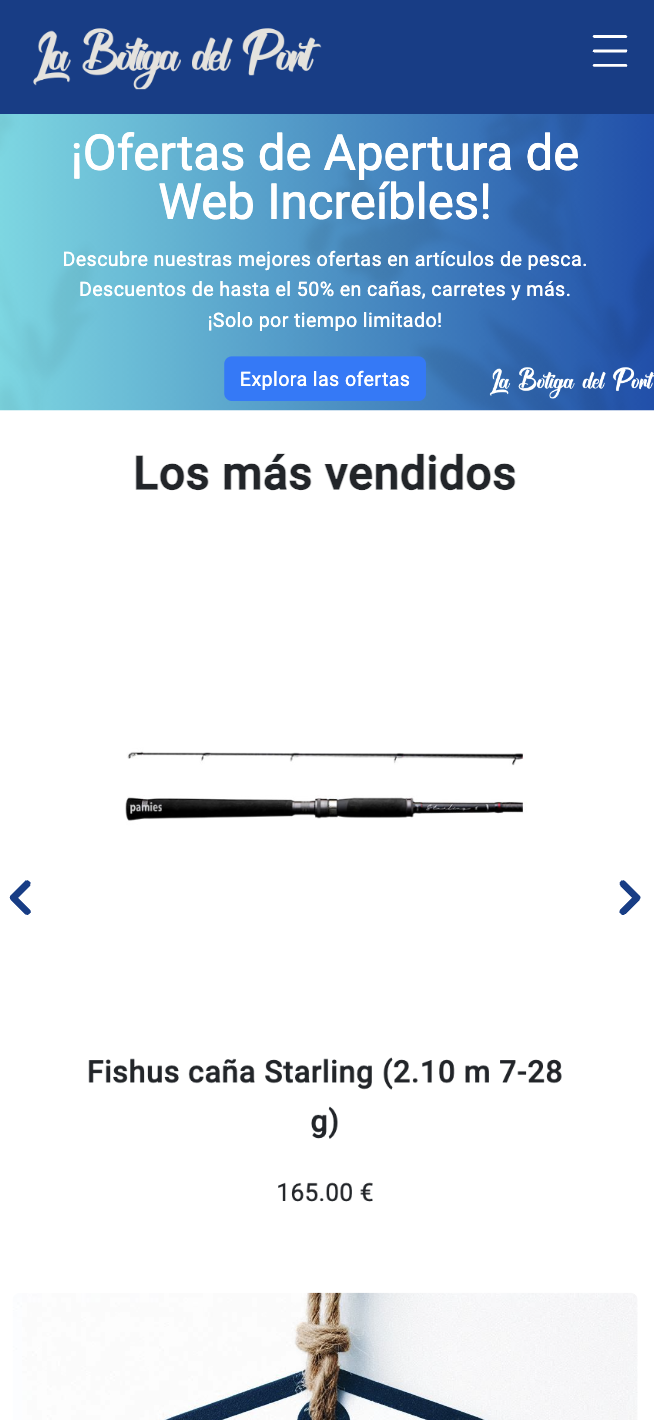
\includegraphics[scale=0.35]{./Images/vistaMobile.png}
\caption{Vista general en mobile} Fuente: Elaboración propia.

\label{fig:fig2}

\end{center}
\end{figure}

\begin{figure}[H]
\begin{center}
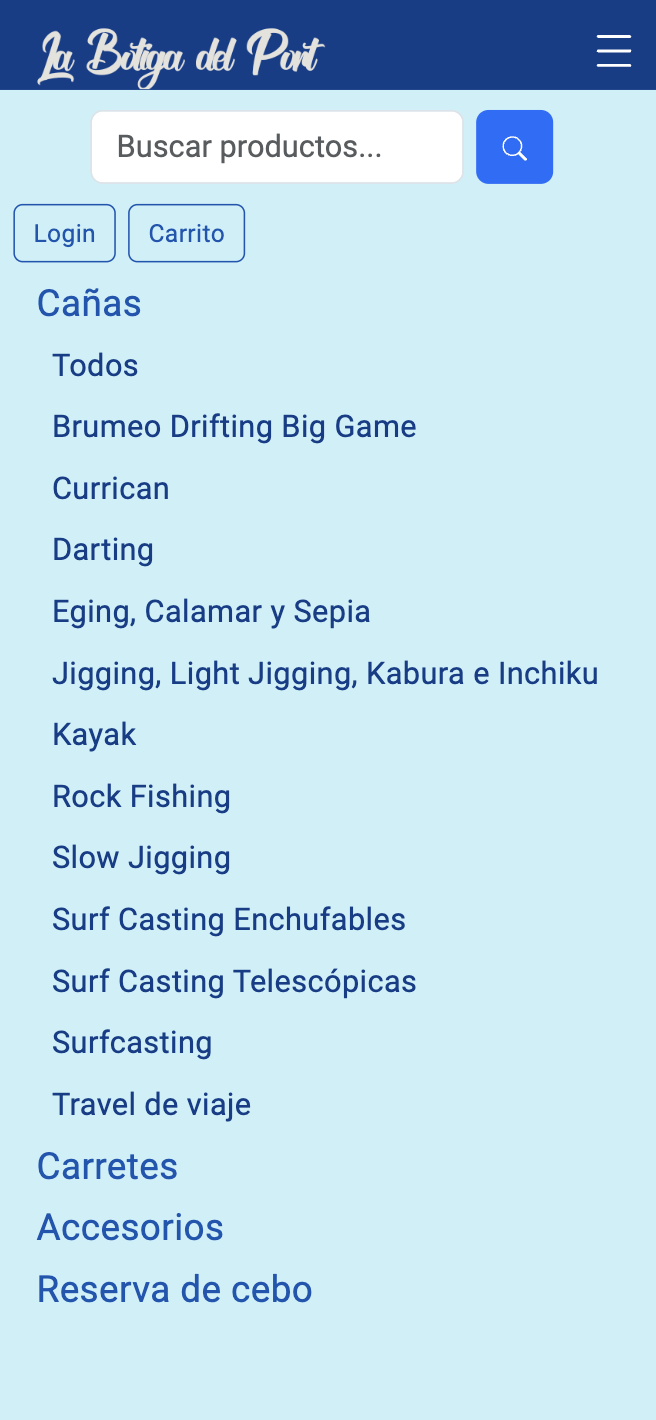
\includegraphics[scale=0.35]{./Images/vistaMobileOpen.png}
\caption{Vista del menú en mobile} Fuente: Elaboración propia.

\label{fig:fig2}

\end{center}
\end{figure}

\section{Uso de la aplicación}\label{sec:apartado}

El uso de la aplicación y las funcionalidades que esta ofrece están directamente basados en los requisitos funcionales establecidos al comienzo del proyecto. Estas funcionalidades han sido diseñadas para garantizar que la aplicación cumpla con los objetivos planteados y proporcione una experiencia de usuario eficaz y coherente.

\subsection{Login y registro de usuario}\label{subsec5.2.1}
    
El login y el registro son funciones fundamentales que permiten a los usuarios interactuar con la aplicación de manera segura y personalizada. El proceso de registro permite la creación de un perfil único para cada usuario, lo que les da acceso a funciones avanzadas como realizar pedidos, reservar cebo y gestionar sus datos. Una vez registrados, los usuarios pueden acceder a su cuenta a través de la funcionalidad de login, la cual asegura que solo aquellos con credenciales válidas puedan acceder a estas funciones específicas. Esto garantiza un control adecuado sobre el acceso y proporciona una experiencia de usuario segura y eficiente dentro de la aplicación.

\vspace{0.5cm}

Adicionalmente, cuando un usuario inicia sesión con credenciales de administrador, la aplicación presenta una vista diferente diseñada específicamente para la gestión administrativa. Esta vista del administrador permite al usuario gestionar diversos aspectos críticos de la aplicación, como productos, pedidos y reservas de cebo. La interfaz administrativa proporciona herramientas para controlar y modificar elementos visuales, gestionar inventarios, y supervisar el estado de las reservas y pedidos. Esta separación entre vistas asegura que las funciones de administración estén claramente diferenciadas y accesibles solo para los usuarios con permisos adecuados, optimizando así la eficiencia y la seguridad en la gestión de la aplicación.

\subsection{Productos}\label{subsec5.2.2}

La gestión de productos dentro de la aplicación es una funcionalidad clave que permite a los usuarios explorar y seleccionar artículos de manera eficiente. A través de la vista de productos, los usuarios pueden navegar por distintas subcategorías, como cañas, carretes y accesorios, o por características específicas como novedades, ofertas y liquidación. Cada producto está presentado con imágenes representativas, descripciones detalladas, y un precio visible, lo que facilita la toma de decisiones de compra. Además, la aplicación permite a los usuarios seleccionar la cantidad de un producto que desean añadir al carrito, haciendo que el proceso de compra sea sencillo e intuitivo.

\vspace{0.5cm}

Los productos añadidos al carrito pueden ser gestionados desde la vista de carrito, donde los usuarios pueden ver todos los artículos que han seleccionado. En esta vista, es posible modificar la cantidad de cada producto o eliminar artículos según sea necesario. A la derecha, se muestra un resumen con la suma total del precio de los productos en el carrito. Además, se ofrece la opción de añadir un código de descuento; si el código es válido, se aplicará automáticamente el descuento correspondiente. En caso contrario, el sistema informará al usuario si el código es inválido o si ha caducado, proporcionando una experiencia de compra transparente y eficaz.

\vspace{0.5cm}

Una vez que el cliente ha añadido los productos deseados al carrito y aplicado cualquier código de descuento, puede proceder al pago presionando el botón de "Pagar". En ese momento, el sistema genera una confirmación de pedido, que se muestra en pantalla con un resumen de los productos adquiridos, sus cantidades y el precio total. Además, una copia de esta confirmación es enviada automáticamente al correo electrónico del cliente, proporcionando un registro del pedido. Simultáneamente, el administrador de la tienda recibe también una notificación por correo electrónico con los detalles del pedido, permitiendo una preparación rápida y eficiente del mismo.

\vspace{0.5cm}

En la pestaña de perfil de la aplicación, el cliente tiene acceso a una vista completa de todos los pedidos que ha realizado a lo largo del tiempo. En esta sección, el cliente puede revisar los detalles de cada uno de sus pedidos pasados, proporcionando un historial claro y organizado. Además, desde la misma pestaña, el usuario puede gestionar sus datos personales, como el nombre, la dirección de correo y otros detalles relevantes para sus futuras compras.

\vspace{0.5cm}

Para el usuario con credenciales de administrador, la aplicación ofrece funcionalidades adicionales que permiten una gestión completa del catálogo de productos. El administrador pueden editar los detalles de cualquier producto, así como eliminar o añadir nuevos artículos a la tienda. También tienen la capacidad de marcar productos como liquidación o novedad, lo que afecta directamente a cómo estos artículos se muestran en las subcategorías específicas de la aplicación. Si un producto tiene un precio con descuento, automáticamente aparece en la subsección de ofertas, asegurando que los usuarios puedan identificar fácilmente las promociones disponibles.

\vspace{0.5cm}

Además de la gestión de productos, los administradores pueden modificar aspectos visuales clave de la aplicación. Esto incluye la capacidad de editar el banner principal, cambiando su texto, imagen y enlace, lo que permite mantener el contenido de la tienda siempre actualizado y relevante. Los administradores también pueden seleccionar qué seis productos aparecen en el carrusel de la página principal, destacando los artículos que se deseen promover. Asimismo, el adminsitrador tienen la posibilidad de gestionar los códigos de descuento, pudiendo añadir nuevos, modificar su nombre o la fecha en que están vigentes, y eliminar aquellos que ya no son necesarios. Estas herramientas de personalización aseguran que la tienda pueda adaptarse rápidamente a nuevas campañas de marketing o promociones, manteniendo una experiencia de usuario dinámica y atractiva.


\subsection{Reserva de Cebo}\label{subsec5.2.3}

La funcionalidad de reserva de cebo dentro de la aplicación ofrece a los clientes una forma sencilla y eficiente de seleccionar y reservar cebo para recoger en tienda en una fecha posterior. En la subpágina dedicada a la reserva de cebo, se muestran todos los productos disponibles de esta categoría, cada uno acompañado de su imagen representativa, nombre y precio, facilitando así la exploración de las opciones disponibles. Junto a cada producto, el cliente encontrará botones para seleccionar la cantidad de cebo que desea reservar.

\vspace{0.5cm}

En la parte superior de esta vista, se ofrece un campo de entrada tipo calendario, que permite al cliente seleccionar la fecha en la que desea recoger su reserva. Esta fecha debe ser siempre posterior al día actual, lo que garantiza que el administrador disponga del tiempo necesario para preparar el pedido. Una vez seleccionados los productos y la fecha de recogida, el cliente puede proceder a realizar la reserva mediante el botón de "Reservar cebo". 

\vspace{0.5cm}

Para continuar con la reserva, el cliente debe estar registrado y haber iniciado sesión. Si no lo ha hecho, la aplicación redirigirá al cliente a la página de inicio de sesión, donde podrá autenticarse o crear una cuenta si aún no tiene una. Una vez autenticado, el cliente será redirigido de nuevo a la página de resumen de su reserva, donde podrá revisar y modificar los productos seleccionados, la cantidad de cada uno y la fecha de recogida. Cuando esté satisfecho con los detalles de su reserva, podrá confirmarla.

\vspace{0.5cm}

Tras la confirmación de la reserva, el cliente verá una pantalla de confirmación y, además, recibirá un correo electrónico con los detalles de la reserva, para tener un registro permanente de la misma. De manera simultánea, el administrador de la tienda también recibirá un correo electrónico con los detalles de la reserva, lo que le permitirá preparar con antelación los pedidos que se recogerán en el futuro.

\vspace{0.5cm}

En la interfaz de administración, el sistema ofrece una vista completa de todas las reservas de cebo realizadas por los clientes. El administrador puede visualizar cada reserva con sus detalles, como el nombre del cliente, los productos reservados, la cantidad de cada uno y la fecha de recogida. Esta vista incluye filtros que permiten al administrador organizar las reservas según sean pasadas o futuras, o bien buscar reservas específicas por el nombre del cliente. 

\vspace{0.5cm}

Cuando un cliente acude a la tienda para recoger su cebo, el administrador puede marcar la reserva como "recogida", lo que facilita el seguimiento de las reservas completadas y garantiza un control eficaz sobre los pedidos. De este modo, la funcionalidad asegura que tanto el cliente como el administrador puedan gestionar el proceso de reserva y recogida de forma rápida, clara y eficiente, proporcionando una experiencia de usuario fluida y un control administrativo preciso.